\documentclass[a4paper]{article}
\usepackage[utf8]{inputenc}
\usepackage{alphabeta}
\usepackage{graphicx}
\usepackage[section]{placeins}
\usepackage{float}
\usepackage{amsmath}
\usepackage{listings}
\usepackage{xcolor}
\usepackage{amsmath}
\usepackage{extarrows}
\usepackage{amssymb}
\usepackage{verbatim}
\usepackage{enumerate}
\usepackage{eurosym}
\usepackage{svg}
\usepackage{varwidth}

\definecolor{codegreen}{rgb}{0,0.6,0}
\definecolor{codegray}{rgb}{0.5,0.5,0.5}
\definecolor{codepurple}{rgb}{0.58,0,0.82}
\definecolor{backcolour}{rgb}{0.95,0.95,0.92}

\lstdefinestyle{mystyle}{
    backgroundcolor=\color{backcolour},   
    commentstyle=\color{codegreen},
    keywordstyle=\color{magenta},
    numberstyle=\tiny\color{codegray},
    stringstyle=\color{codepurple},
    basicstyle=\ttfamily\footnotesize,
    breakatwhitespace=false,         
    breaklines=true,                 
    captionpos=b,                    
    keepspaces=true,                 
    numbers=left,                    
    numbersep=5pt,                  
    showspaces=false,                
    showstringspaces=false,
    showtabs=false,                  
    tabsize=2
}

\lstset{style=mystyle}

\setlength{\parindent}{0pt}
\setlength{\parskip}{1em}
\setlength{\jot}{4mm}

\title{Συστήματα Αναμονής \\ 3η εργαστηριακή άσκηση}
\author{Νικόλαος Παγώνας, el18175}
\date{}

\begin{document}

\maketitle

\subsection*{Προσομοίωση συστήματος Μ/Μ/1/10}

\subsection*{(1)}

\begin{minipage}{\textwidth}

Εκτυπώνουμε τις πρώτες 30 μεταβάσεις για λ = \{1,5,10\} προκειμένου να επιβεβαιώσουμε την ορθή λειτουργία της προσομοίωσης.\\

Για λ = 1, μ = 5:
\small
\verbatiminput{images/trace1.txt}
\normalsize
\end{minipage}

\begin{minipage}{\textwidth}
Για λ = 5, μ = 5:
\small
\verbatiminput{images/trace2.txt}
\normalsize
\end{minipage}


\begin{minipage}{\textwidth}
Για λ = 10, μ = 5:
\small
\verbatiminput{images/trace3.txt}
\normalsize
\end{minipage}

\begin{minipage}{\textwidth}
\subsection*{(2)}

Χρησιμοποιούμε την προσομοίωση που φτιάξαμε για να παρακολουθήσουμε τη σύγκλιση των ζητούμενων μεγεθών. Η σύγκλιση είναι εγγυημένη καθώς πρόκειται για ουρά πεπερασμένης χωρητικότητας. Σημειώνεται ότι οι οριζόντιες μαύρες γραμμές αποτελούν την τιμή-στόχο της σύγκλισης και προέκυψαν μέσω της εντολής qsmmmk() του πακέτου queueing, η χρήση της οποίας έγινε καθαρά και μόνο για επαλήθευση των αποτελεσμάτων. \\

\textbf{Για λ = 1, μ = 5:} \\

Εργοδικές πιθανότητες των καταστάσεων του συστήματος:

\verbatiminput{images/prob1.txt}

\begin{figure}[H]
	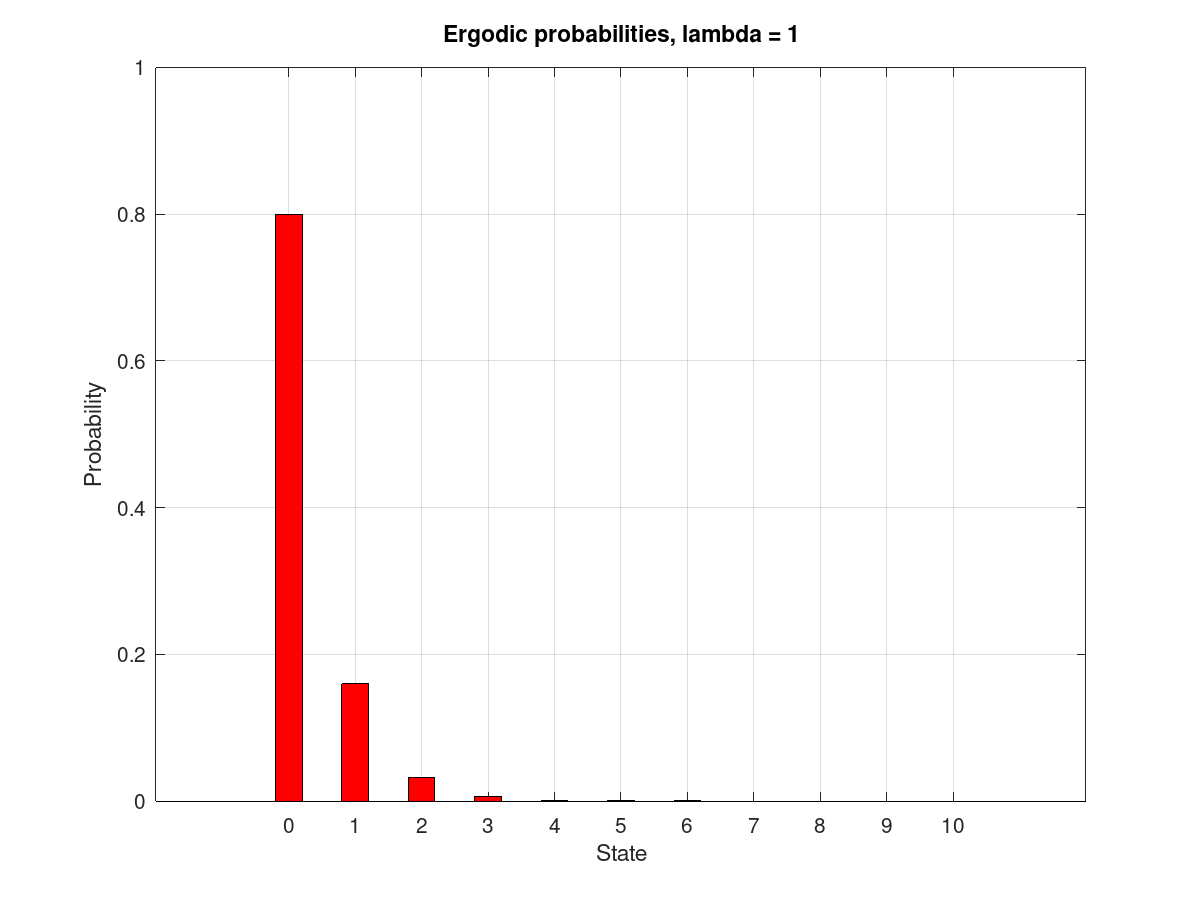
\includegraphics[width=\textwidth]{images/prob1.png}
\end{figure}

\end{minipage}

\begin{minipage}{\textwidth}
Πιθανότητα απόρριψης πελάτη από το σύστημα:

\verbatiminput{images/pblocking1.txt}

Εξέλιξη του μέσου αριθμού πελατών:

\begin{figure}[H]
	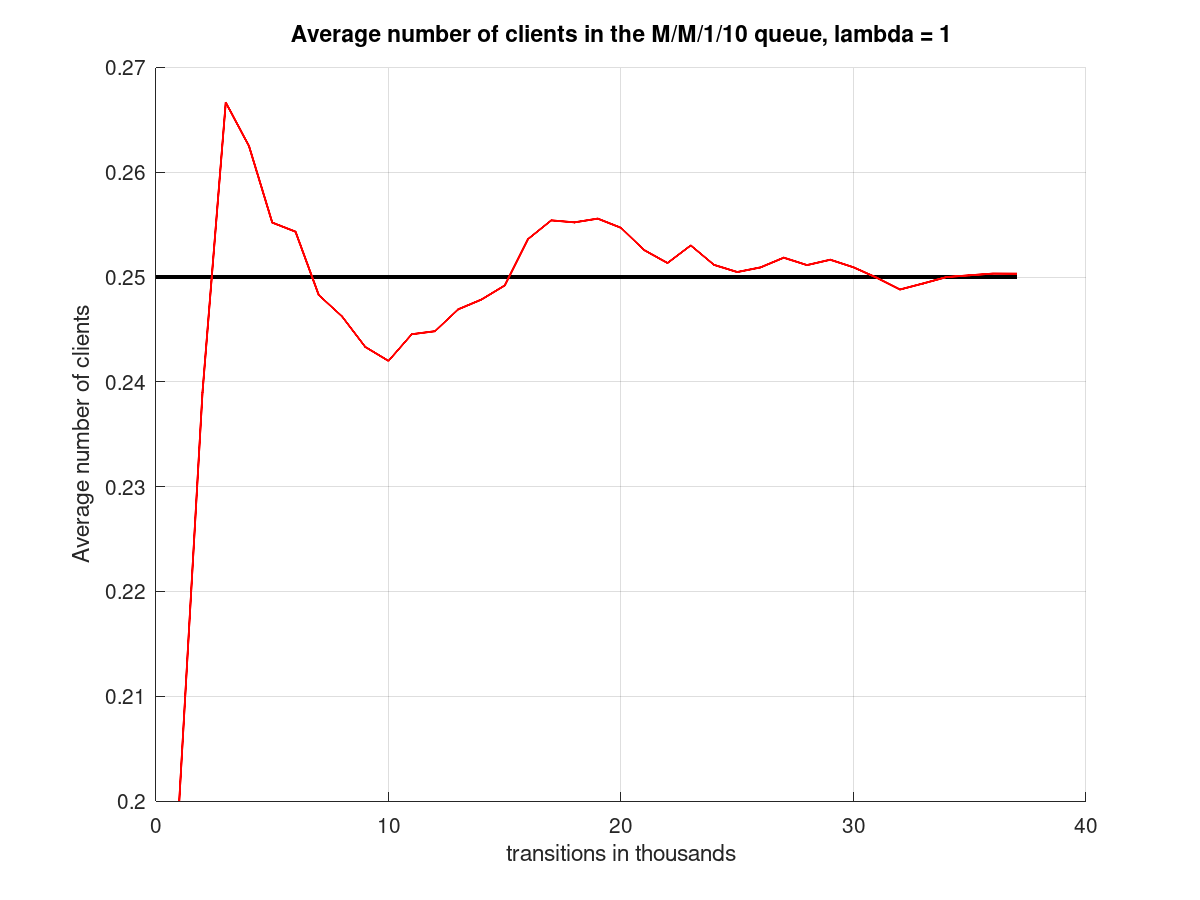
\includegraphics[width=\textwidth]{images/clients1.png}
\end{figure}
\end{minipage}

\begin{minipage}{\textwidth}
Εξέλιξη του μέσου χρόνου καθυστέρησης:

Από τον νόμο του Little: $ E[T] = \dfrac{E[n(t)]}{λ(1-P[\text{blocking}])} $

\begin{figure}[H]
	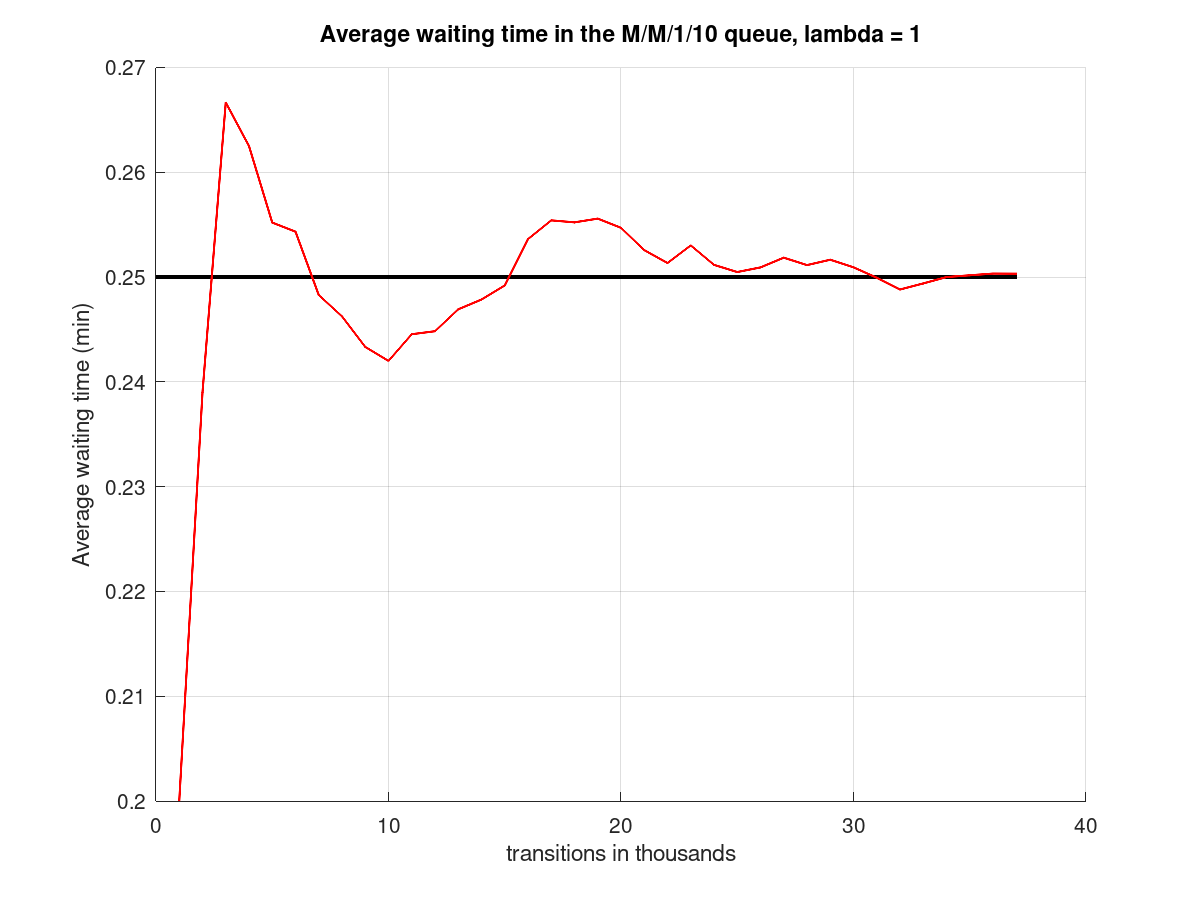
\includegraphics[width=\textwidth]{images/time1.png}
\end{figure}

\end{minipage}

\begin{minipage}{\textwidth}

\textbf{Για λ = 5, μ = 5:} \\

Εργοδικές πιθανότητες των καταστάσεων του συστήματος:

\verbatiminput{images/prob2.txt}

\begin{figure}[H]
	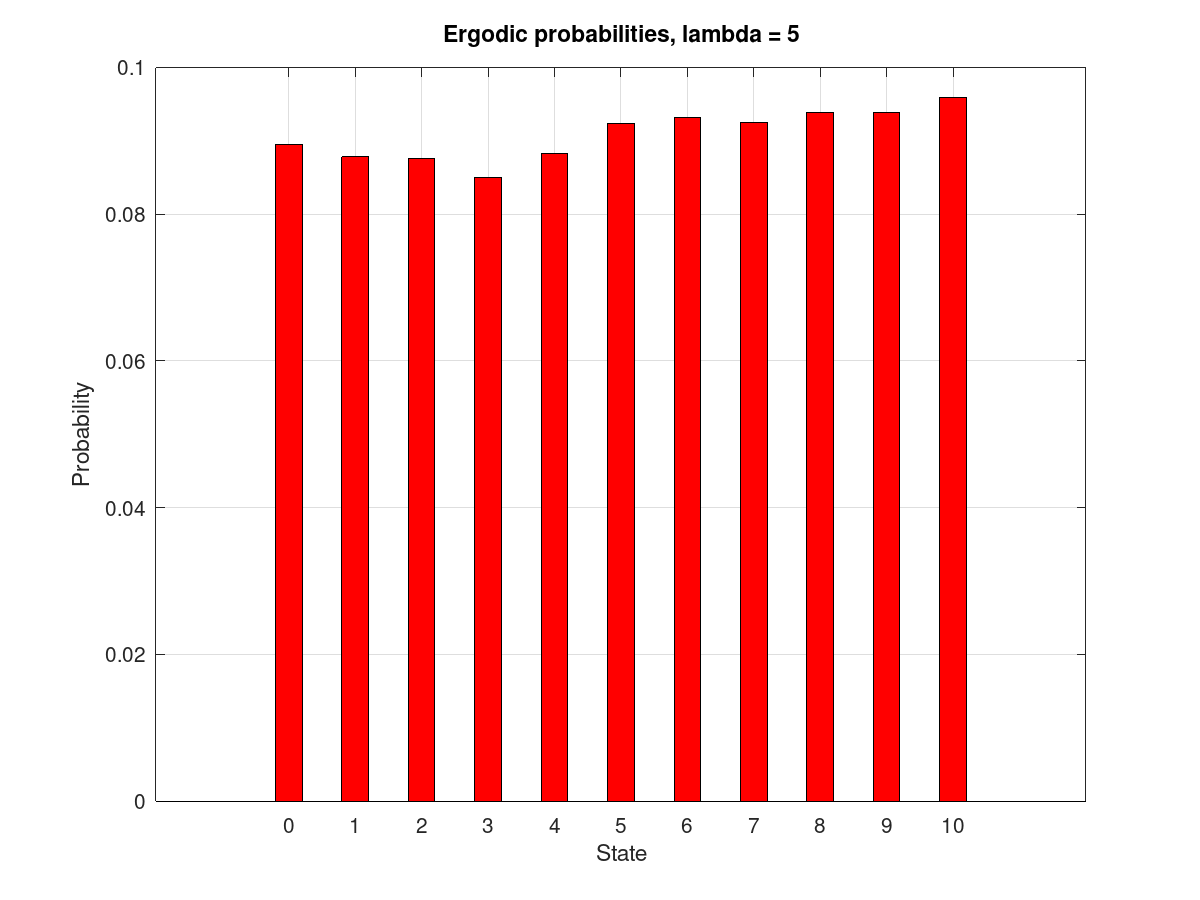
\includegraphics[width=\textwidth]{images/prob2.png}
\end{figure}

Πιθανότητα απόρριψης πελάτη από το σύστημα:

\verbatiminput{images/pblocking2.txt}
\end{minipage}

\begin{minipage}{\textwidth}
Εξέλιξη του μέσου αριθμού πελατών:

\begin{figure}[H]
	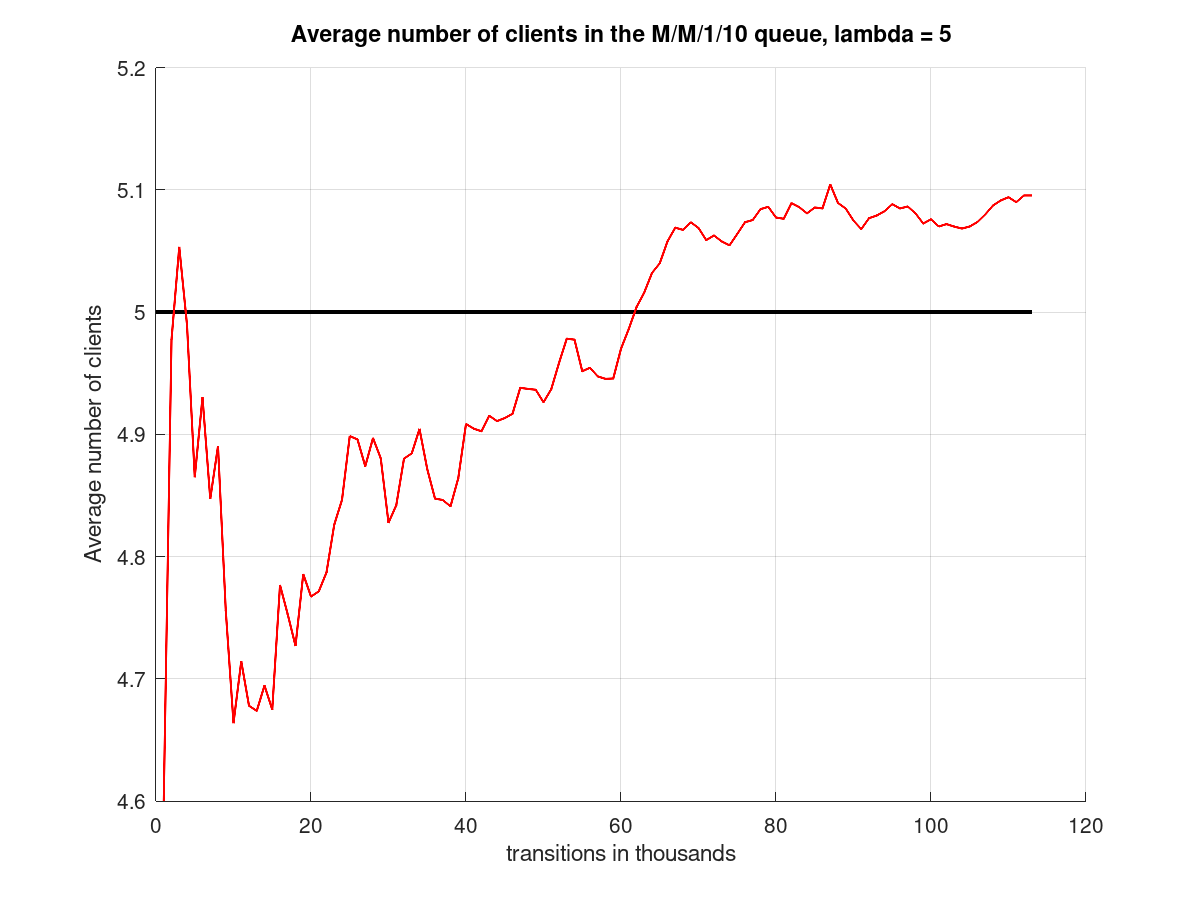
\includegraphics[width=\textwidth]{images/clients2.png}
\end{figure}

Εξέλιξη του μέσου χρόνου καθυστέρησης: \\

Από τον νόμο του Little: $ E[T] = \dfrac{E[n(t)]}{λ(1-P[\text{blocking}])} $

\begin{figure}[H]
	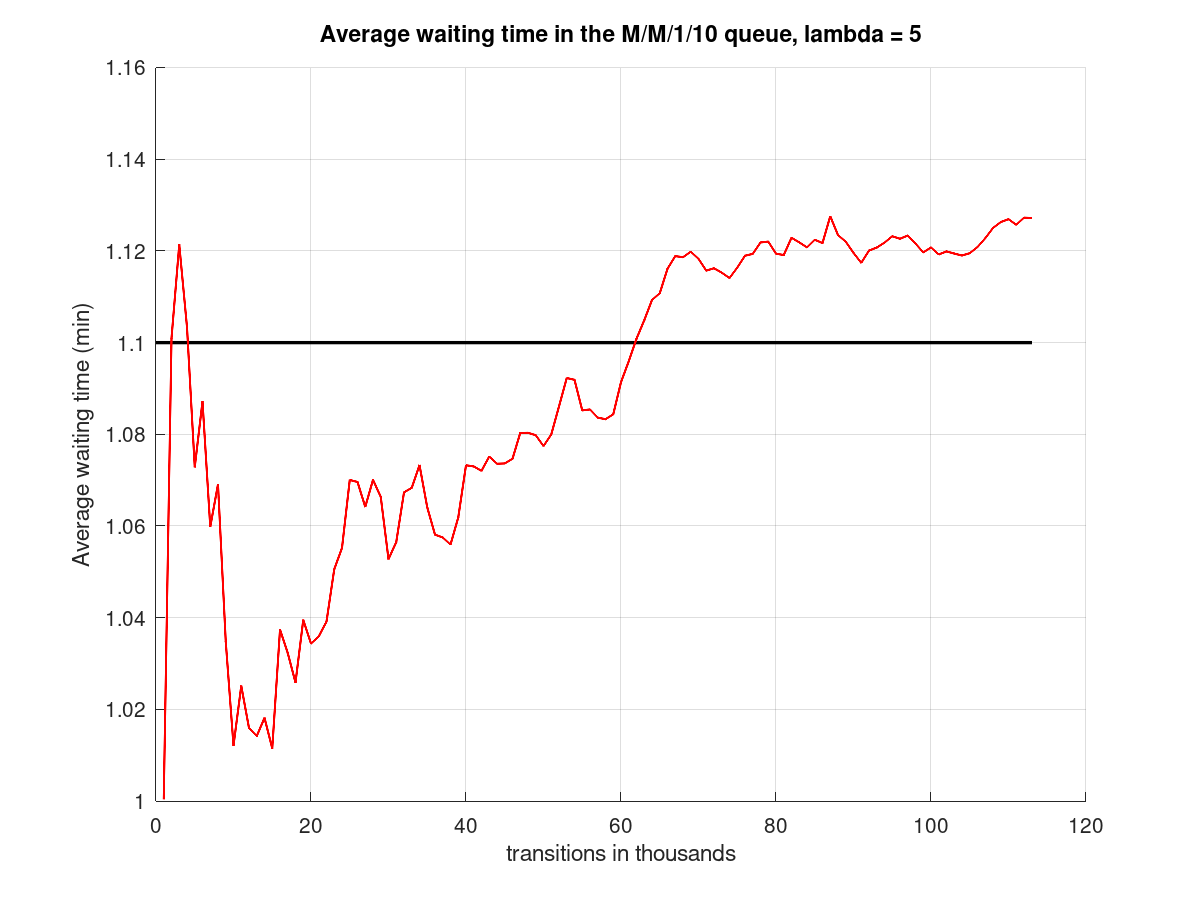
\includegraphics[width=\textwidth]{images/time2.png}
\end{figure}
\end{minipage}

\begin{minipage}{\textwidth}
\textbf{Για λ = 10, μ = 5:} \\

Εργοδικές πιθανότητες των καταστάσεων του συστήματος:

\verbatiminput{images/prob3.txt}

\begin{figure}[H]
	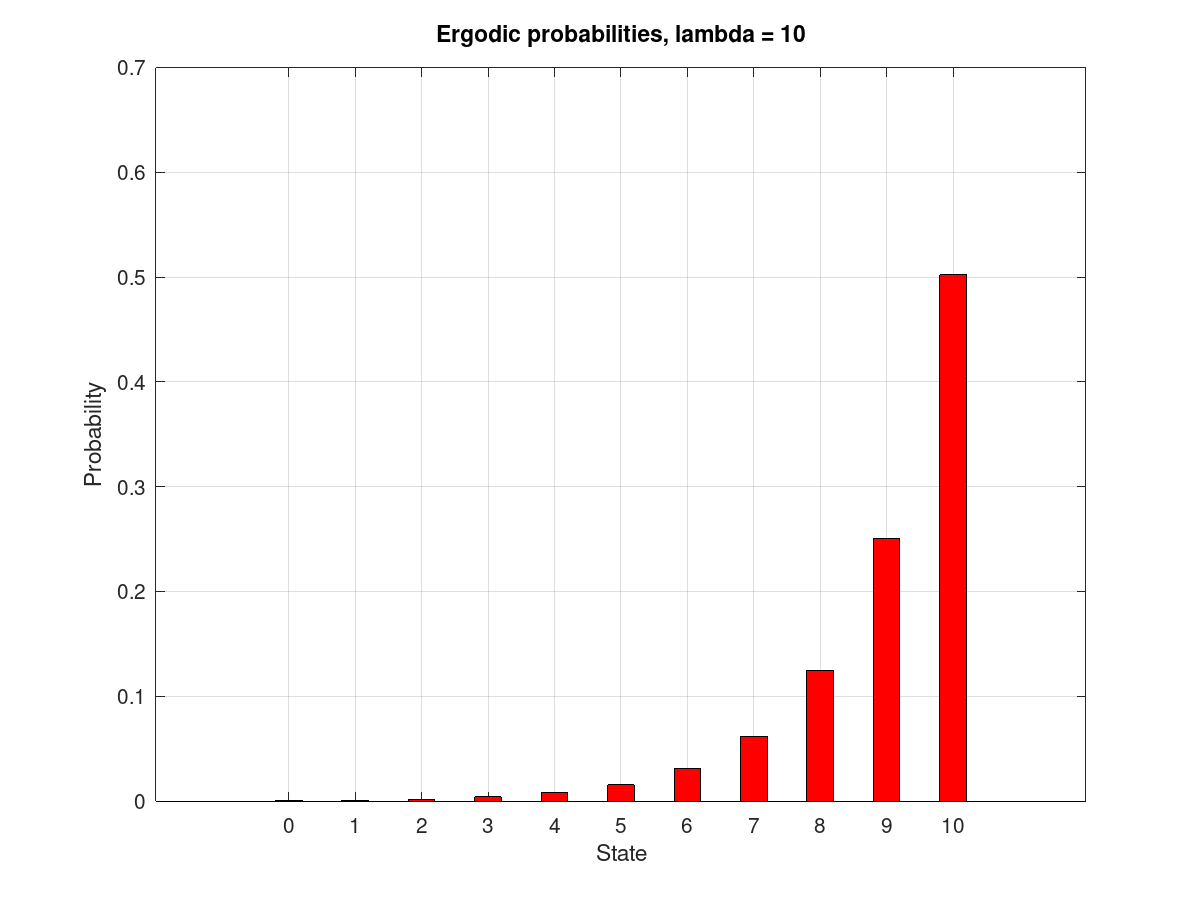
\includegraphics[width=\textwidth]{images/prob3.png}
\end{figure}

Πιθανότητα απόρριψης πελάτη από το σύστημα:

\verbatiminput{images/pblocking3.txt}

\end{minipage}

\begin{minipage}{\textwidth}
Εξέλιξη του μέσου αριθμού πελατών:

\begin{figure}[H]
	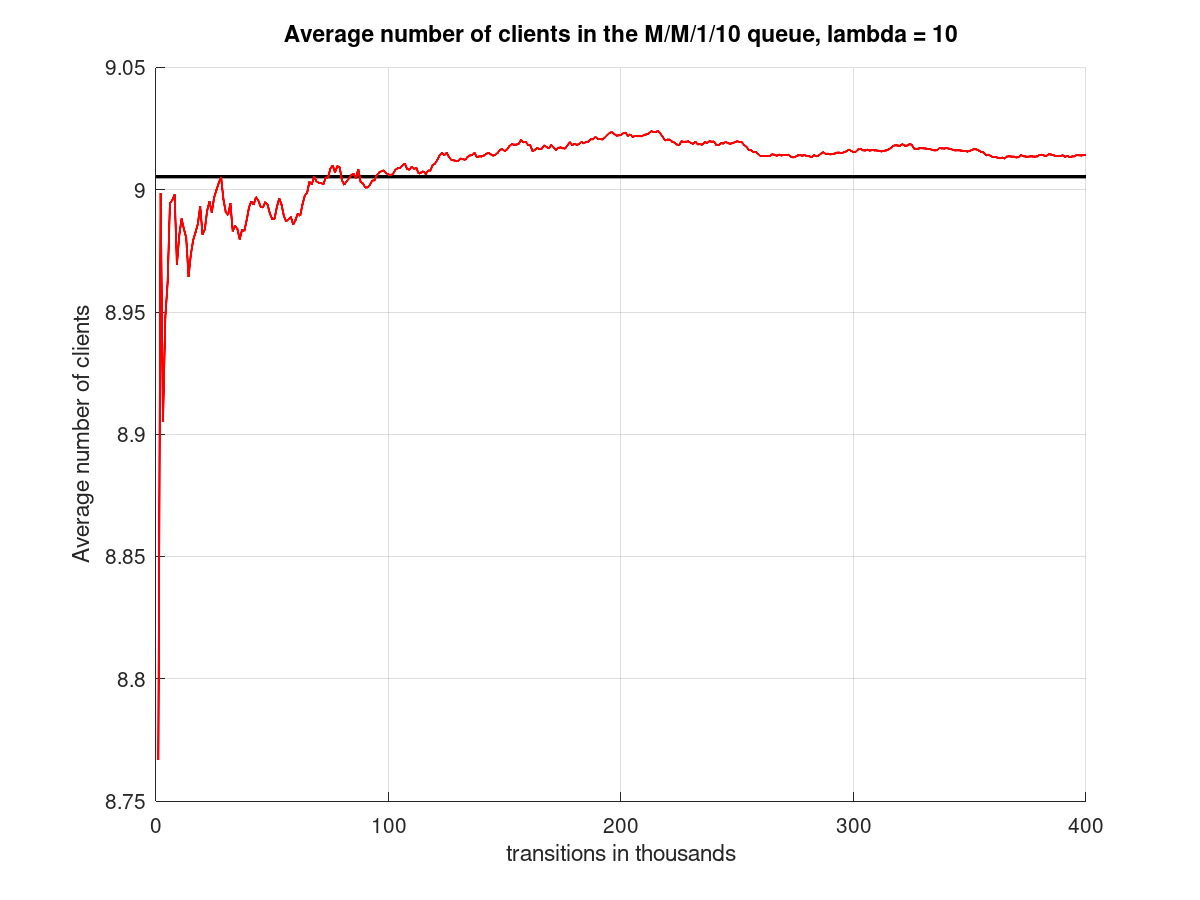
\includegraphics[width=\textwidth]{images/clients3.png}
\end{figure}

Εξέλιξη του μέσου χρόνου καθυστέρησης:

Από τον νόμο του Little: $ E[T] = \dfrac{E[n(t)]}{λ(1-P[\text{blocking}])} $

\begin{figure}[H]
	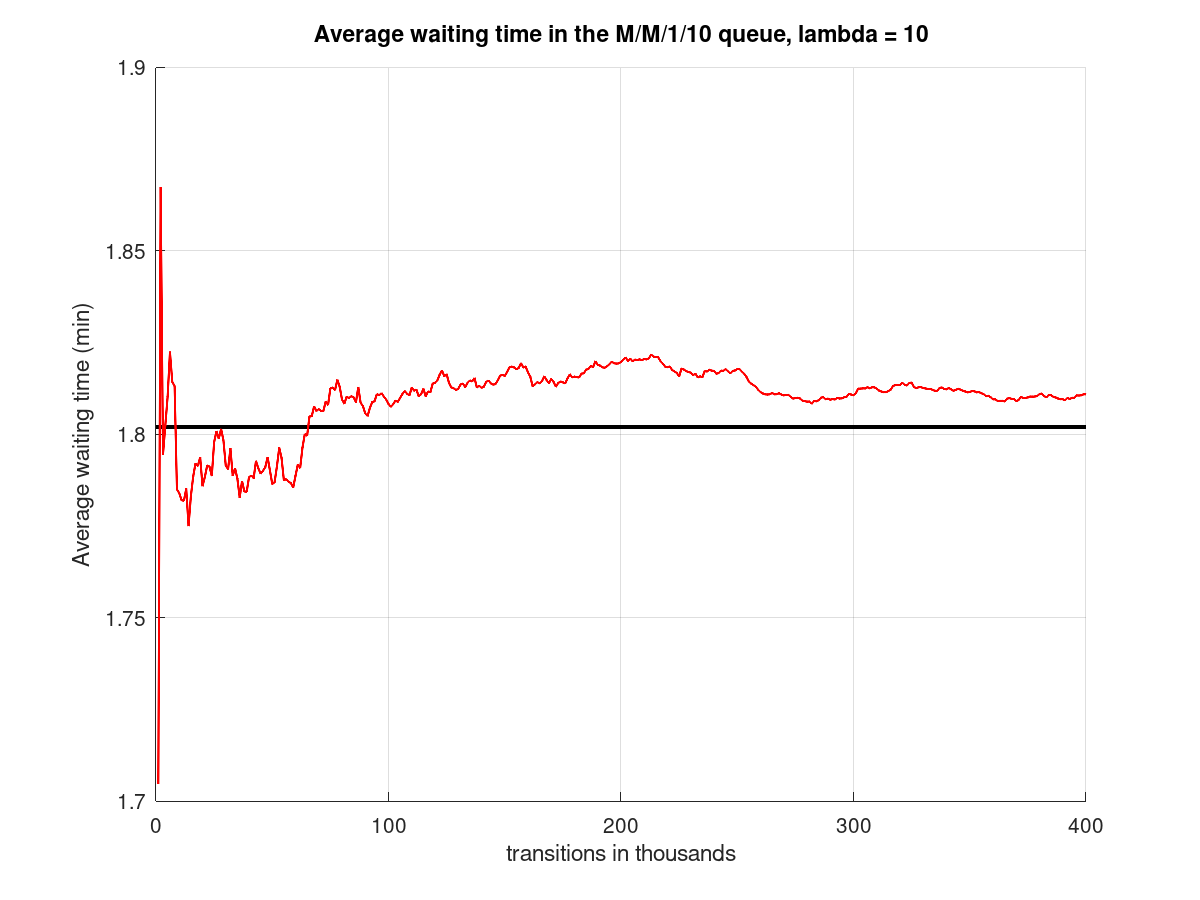
\includegraphics[width=\textwidth]{images/time3.png}
\end{figure}

\end{minipage}

\subsection*{(3)}

Παρατηρούμε ότι όσο μεγαλώνει το λ, η προσομοίωση χρειάζεται περισσότερο χρόνο για να φτάσει στη σύγκλιση. Αυτό συμβαίνει διότι ο εξυπηρετητής δεν μπορεί να ικανοποιήσει με την ίδια επάρκεια τον ολοένα και αυξανόμενο φόρτο αφίξεων, με αποτέλεσμα να επισκεπτόμαστε πιο συχνά τις τελευταίες καταστάσεις. Έτσι, απαιτείται επιπλέον χρόνος προκειμένου:
 
\begin{itemize}
	\item να μεταβούμε στις τελευταίες καταστάσεις (και ενδεχομένως να αρχίσουμε να απορρίπτουμε πελάτες)
	\item οι τελευταίες καταστάσεις να συγκλίνουν κι αυτές. 
\end{itemize}

Πριν που το λ ήταν μικρότερο, η επισκεψιμότητα των τελευταίων καταστάσεων, και άρα η διαφοροποίησή τους μεταξύ διαδοχικών convergence tests ήταν κι αυτή μικρότερη. Λογικό είναι λοιπόν η διάρκεια της προσομοίωσης να αυξηθεί.

Επίσης, παρατηρώντας προσεκτικά τα διαγράμματα για λ = \{1,5,10\}, διακρίνουμε κάποια μεταβατικά φαινόμενα, δηλαδή ο μέσος αριθμός πελατών παρουσιάζει μεγάλες διακυμάνσεις αρχικά, μέχρι να σταθεροποιηθεί. Συγκεκριμένα, για λ = \{1,5,10\} οι διακυμάνσεις παρατηρούνται για τα πρώτα \{15.000, 30.000, 40.000\} transitions αντίστοιχα (περίπου). Επομένως, ένας τρόπος να επιταχύνουμε την προσομοίωση είναι να μην κάνουμε έλεγχο σύγκλισης μέχρι να φτάσουμε έναν ικανοποιητικό αριθμό transitions (15.000-40.000, ανάλογα την τιμή του λ) αφού βλέπουμε ότι πιθανότατα θα είναι πολύ νωρίς για να έχει συγκλίνει η προσομοίωση. 

\subsection*{(4)}

Αν είχαμε $ μ_i = μ \cdot (i+1), \text{ με } μ = 1 $, θα έπρεπε να προσέξουμε ότι το threshold πλέον αλλάζει κάθε φορά που βρισκόμαστε σε άλλη κατάσταση. Έτσι, η ανάθεση του threshold πρέπει να μπει μέσα στο while-loop, ώστε αυτό να αλλάζει σε κάθε transition, και όχι μόνο την πρώτη φορά που τρέχουμε την προσομοίωση. Κατά τα άλλα, θα έχουμε:

\[
	threshold = \frac{λ_i}{λ_i+μ_i} = \frac{λ_i}{λ_i+i+1}, \text{ αφού μ = 1}
\]

\subsection*{Παράρτημα Κώδικα}
\lstinputlisting[language=octave]{simulation.m}
\end{document}
